\ifdefined\XeTeXrevision\else\pdfoutput=1\fi
\documentclass[11pt]{article}
\usepackage[margin=1in]{geometry}
\usepackage{booktabs}
\usepackage{amsmath}
\usepackage{graphicx}
\usepackage{xcolor}
\usepackage{hyperref}
\usepackage{microtype}
\hypersetup{
  colorlinks=true,
  linkcolor=blue!60!black,
  citecolor=blue!60!black,
  urlcolor=blue!60!black,
  pdftitle={One Mouth, One Mode},
  pdfauthor={Franci Penov},
}
\title{One Mouth, One Mode:\\Mode Exclusion and the Teacher-Forced/Free-Run Gap\\in a Self-Bridged 4B}
\author{Franci Penov \\ kortexa.ai \\ \texttt{francip@kortexa.ai}}
\date{2026-08-08}

\begin{document}
\maketitle

\begin{abstract}
The self-bridge program trains a frozen language model to write a
256-dimensional latent note that its own next pass reads.  At 0.8B the
channel exists: a nine-check promotion gate passes at all three seeds, with
greedy decode recovering 16 of 16 private contents from an empty context.
This note documents what happened when the construction was promoted to a 4B
host carrying sensor blocks --- four registered experiments stopped in
sequence, and the post-mortem is one phenomenon.  Across
1,056 informed-teacher decodes, recalling the first act fired
40 times, expressing the second act's state fired
499 times, and \emph{both never fired together} ---
independence predicts 19 co-occurrences
($P(0) \approx 6\times 10^{-9}$).  At 4B, recall and presence are
mutually exclusive modes of one utterance.  Authoring the joint behaviour
does not rescue it: a packet trained by teacher forcing to a
machine-validated composed target fits it (final token accuracy
0.95--1.00, target-exact up to 1.00) and
free decode carries none of it (0.000 at 12 (pair, seed)
cells and five doses, floors included).  On-policy exposure does not move it: scheduled sampling --- student-sampled prefixes with only the authored target's suffix supervised, mixing ratio annealed 0$\to$1 --- leaves free-run carry at 0.000 across all 12 cells and 5 doses, even though the packet learns to complete the target from the student's own prefixes.  Every integrity
check --- zero-dose bit-exactness, byte-identical base weights, a
plumbing-asserted fresh context --- held throughout, so the zeros are
measurements, not accidents.
\end{abstract}

\section{Why this note exists}

The program's model-of-models relay showed that an untrained pass boundary
loses everything --- the KV cache demonstrably holds a large unread signal
--- and that \emph{training} an emitter/receiver pair turns the same
boundary into a working channel.  The self-bridge asks the mirror question:
can a model write a note to \emph{itself}?  The serving stake is concrete:
per-turn state without retained KV --- the cache is gigabytes and provably
unread; the note is 256 floats.

Stage S1 answered the architecture question cheaply and affirmatively at
0.8B.  A frozen Qwen3.5-0.8B wrote a 256-float packet from its own layer-19
residual; its next pass, in a fresh context with no cache and no
instruction, answered with the private content: held-out top-1 1.000 at
every seed, shuffled packets at 0.000, and the registered nine-check gate
green three times over.  The channel exists, and it is message-dependent ---
with the topic partner's packet the model says the \emph{partner's} word.

Stage S2 promoted the construction to the program's working venue: a frozen
Qwen3.5-4B carrying March r4 sensor blocks (\texttt{temporal},
\texttt{self}, \texttt{geo}), where the note must substitute for a
missing two-turn history --- block A answers in pass 1, block B acts in pass
2, and the packet must carry A's content across.  Four registered
experiments then stopped in sequence.  None of the stops was a harness
failure, and together they resolve into one measured phenomenon.  This note
is the record.

\section{The four stops}

\textbf{S2: the second act is empty.}  The registered objective was v1.10
distillation from an informed teacher --- the same frozen host decoding pass
2 \emph{with the pass-1 exchange present as text}.  The registered
usability rule excluded any teacher item that failed either lane's scorer,
under a two-thirds survival floor.  Survival was
0.0 in every
pair: the informed teacher does its own job (B-function
0.375--0.625) and never restates A's (0.000--0.050).
Worse, block B alone on a null turn --- \texttt{b-solo}, the function the
gate protects --- was 0 of 44 across every pair.  At 35B the same
construction gave 0.400--0.467; the null-turn convention does not transfer
down.

\textbf{S2a: waking is not carrying.}  An amendment replaced the null turn
with a screened bank of eight neutral synthesis prompts.  The screen
confirmed the amendment's mechanism claim --- situation-naming prompts wake
the sleeping block, \texttt{b-solo} rising from 0.000 to 0.417 --- and
refuted its hope: teacher A-carry stayed at 0.000--0.125 per cell against a
registered 0.67 floor.  No prompt was selected; Stage B
never opened.

\textbf{S2b: the exclusion, measured.}  A second amendment gave the
teacher a scaffold the student never sees --- the history \emph{plus} an
explicit recall instruction, three strengths, crossed with the two surviving
prompts.  Usability was 0.000 in all twenty-four cells, and the screen
bought the diagnosis: over all 1,056 teacher decodes, A-carry
fired 40 times, B-function 499 times,
together never (Figure~\ref{fig:exclusion}).  Under independence at the
marginal rates, 18.9 co-occurrences were expected;
observing zero has probability about $6\times 10^{-9}$.  The scaffold
barely moved carry (0.062 to 0.069, weakest to strongest); the backward-looking
prompt moved it three times as much as any instruction --- consistent with a
\emph{mode} the surface can invite but not compound.  Pass-1 quality
compounds the problem (0.27--0.53
under lane A's scorer): the March blocks are weak off their canonical
question, so the note is asked to carry a fact the first act only half
stated.

\begin{table}[t]
\centering
\small
\begin{tabular}{llrrr}
\toprule
scaffold & student prompt & usability & mean A-carry & mean B-function \\
\midrule
T3 & ``So, where were we?'' & 0.000 & 0.069 & 0.497 \\
T1 & ``So, where were we?'' & 0.000 & 0.062 & 0.432 \\
T2 & ``So, where were we?'' & 0.000 & 0.047 & 0.418 \\
T2 & ``Anything I should keep in mind right now?'' & 0.000 & 0.024 & 0.496 \\
T3 & ``Anything I should keep in mind right now?'' & 0.000 & 0.019 & 0.525 \\
T1 & ``Anything I should keep in mind right now?'' & 0.000 & 0.013 & 0.516 \\
\bottomrule
\end{tabular}
\caption{The S2b screen: three teacher scaffolds (T1 weakest to T3 most
explicit) crossed with the two surviving prompts, means over the four
ordered pairs.  Usability --- the fraction of teacher decodes passing both
lanes' scorers --- is exactly zero everywhere, not merely below the
0.67 floor.}
\label{tab:screen}
\end{table}

\begin{figure}[t]
\centering
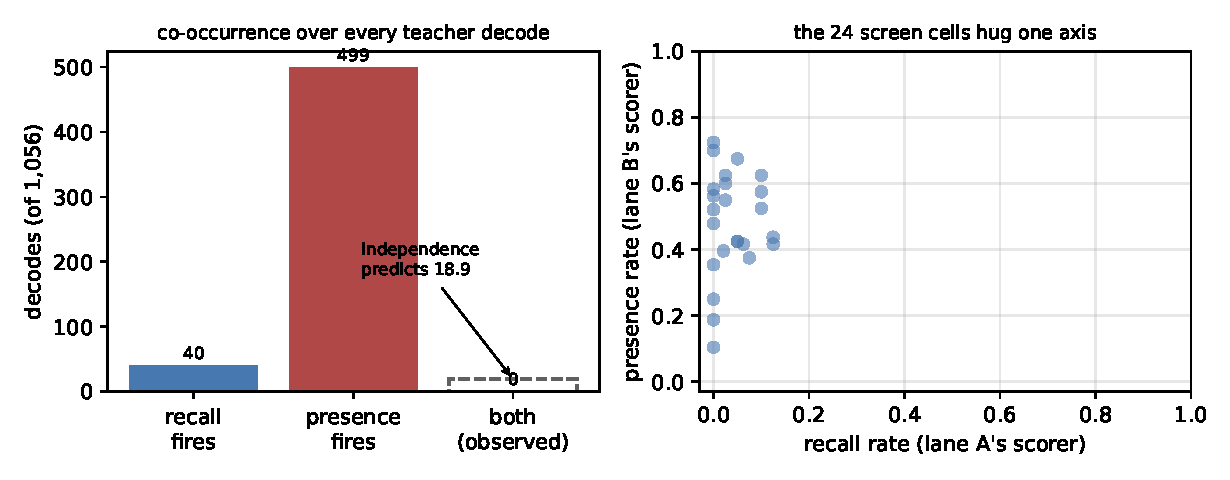
\includegraphics[width=\linewidth]{exclusion.pdf}
\caption{Mode exclusion over the 1,056 S2b teacher decodes.
Left: recall fires 40 times and presence
499 times, but the observed joint count is zero against an
independence prediction of 18.9.  Right: every screen
cell's (recall rate, presence rate) pair --- the cells trade one mode for
the other and never leave the axis.}
\label{fig:exclusion}
\end{figure}

\textbf{S2c: authoring the joint behaviour does not rescue it.}  If no
natural teacher demonstrates the joint utterance, author it: compose
``\{A-content sentence\} \{connective\} \{B-answer\}'' from the lanes'
own banks, with a four-rule machine validation --- each half passes its own
lane's scorer alone, neither passes the other's, every composed target
passes both, no connective carries lane vocabulary --- and train the packet
by teacher-forced transcription (384 steps, batch 8, dose 0.15, three
seeds, four ordered pairs).  The training fits: final token accuracy
0.95--1.00, target-exact up to 1.00 on
the temporal-as-A pairs.  The free run carries none of it: A-carry
0.000 in all 12 cells \emph{and at all five doses}, 0.10
through 0.30, flat (Table~\ref{tab:s2c}, Figure~\ref{fig:gap} left).
Both floors are also at zero, so this is not a threshold artifact; the
shuffled packet is at zero, so nothing leaks; B-function holds near its
in-band solo, so the packet is not destroying the second act --- it is
simply not carrying the first into it.

\begin{table}[t]
\centering
\small
\setlength{\tabcolsep}{4pt}
\begin{tabular}{lrrrrrrr}
\toprule
pair & carry & untrained & diary & B-func. & b-solo & shuffled & target-exact \\
\midrule
\texttt{temporal$>$self} & 0.000 & 0.000 & 0.000 & 0.20--0.30 & 0.300 & 0.000 & 0.50--0.88 \\
\texttt{self$>$temporal} & 0.000 & 0.000 & 0.000 & 0.25--0.42 & 0.417 & 0.000 & 0.12--0.50 \\
\texttt{temporal$>$geo} & 0.000 & 0.000 & 0.000 & 0.30--0.40 & 0.300 & 0.000 & 0.75--0.88 \\
\texttt{geo$>$temporal} & 0.000 & 0.000 & 0.000 & 0.33--0.42 & 0.417 & 0.000 & 0.50--1.00 \\
\bottomrule
\end{tabular}
\caption{S2c at the trained dose: free-run carry is the maximum over every
dose and seed; B-function spans seeds; target-exact spans seeds' final
training steps.  A perfect or near-perfect teacher-forced fit coexists with
zero free-run carry in every row.}
\label{tab:s2c}
\end{table}

\section{Exposure does not rescue it either (S2d)}

The relay ladder has closed a teacher-forced/free-run gap before: v1.7
retargeted its objective at the continuation, and v1.10 added on-policy
sampling, both because a fit was not surviving free decode.  S2d applied the
v1.10 exposure principle to the input: as a mixing ratio anneals linearly
from 0 to 1 over the 384 steps, each training row swaps its opening for the
student's own greedy decode --- sampled through the gate's exact decode
path, packet injected, current bridge --- and supervises only the remainder
of the authored target.  The student's own tokens are context, never
targets.  Everything else ran S2c-verbatim, enforced by construction: the
same driver executes both stages with only the training step swapped.

Exposure was the natural suspect, and it is now measured: training the packet
from the student's own greedy prefixes --- the exact states the free run
visits --- with the target's suffix as the only supervision moves free-run
carry from 0.000 to 0.000.  The schedule itself works: at
intermediate mixing (ratio 0.25--0.75) the student completes the authored
target from its own prefixes at token accuracy
0.80--0.99 (suffix-exact up to
0.88), and 0.68--0.88
at the fully sampled final step.  So the packet can demonstrably
\emph{continue} the joint utterance from wherever the free decode has
wandered --- it can never make the free decode \emph{initiate} it.  The
exclusion binds what the decode starts, not what it can finish, and not the
objective or the training distribution.

\begin{figure}[t]
\centering
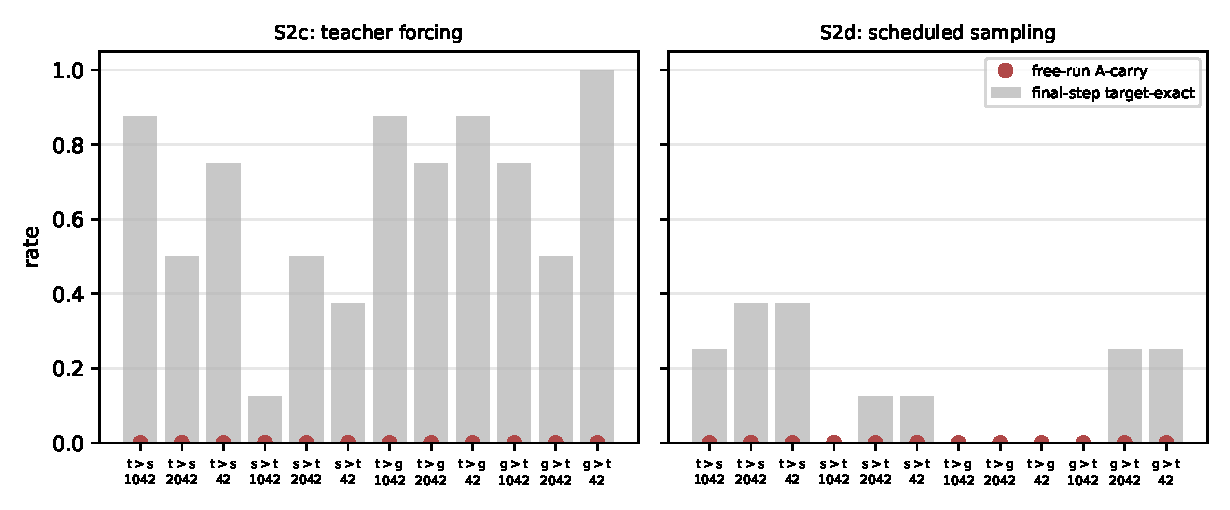
\includegraphics[width=\linewidth]{gap.pdf}
\caption{The fit/free-run gap, per (pair, seed) cell.  Bars: final-step
target-exact --- teacher-forced in S2c, suffix-exact under fully sampled
prefixes in S2d (the harder metric; intermediate-mixing fit is higher, see
text).  Dots: free-run A-carry at the trained dose.}
\label{fig:gap}
\end{figure}

\begin{table}[t]
\centering
\small
\setlength{\tabcolsep}{4pt}
\begin{tabular}{lrrrrrrr}
\toprule
pair & carry & untrained & diary & B-func. & b-solo & shuffled & target-exact \\
\midrule
\texttt{temporal$>$self} & 0.000 & 0.000 & 0.000 & 0.20--0.30 & 0.300 & 0.000 & 0.25--0.38 \\
\texttt{self$>$temporal} & 0.000 & 0.000 & 0.000 & 0.42--0.50 & 0.417 & 0.000 & 0.00--0.12 \\
\texttt{temporal$>$geo} & 0.000 & 0.000 & 0.000 & 0.10--0.30 & 0.300 & 0.000 & 0.00--0.00 \\
\texttt{geo$>$temporal} & 0.000 & 0.000 & 0.000 & 0.42--0.42 & 0.417 & 0.000 & 0.00--0.25 \\
\bottomrule
\end{tabular}
\caption{S2d, same columns as Table~\ref{tab:s2c}.}
\label{tab:s2d}
\end{table}

\section{What the zeros are made of}

The claim ``the packet is the only carrier'' is enforced as plumbing, not
assumed.  A forward pre-hook watches every decoder entry; a \emph{carried}
cache --- one arriving together with a multi-token prefill, the signature of
pass 1's state crossing the boundary --- is an abort, and the count was zero
in every training and evaluation session (S2d's prefix sampling decodes
incrementally inside pass 2, which the guard tallies separately and
permits).  Zero dose with all receivers armed is bit-exact against the
unhooked baseline at every seed.  Base weights are byte-identical after
every session, and the March r4 checkpoints are sha256-verified against the
values the dispatch run recorded before anything is trusted.  The floors
reproduce across sessions to the digit (\texttt{b-solo}
0.300/0.417
under the prompt, diary 0.000--0.025), so the stops are deterministic
properties of the venue, not noise.

\section{What this rules out, and what it leaves}

Taken together, the four stops rule out an entire family of fixes at 4B:
the surface (S2a), the instruction (S2b), the objective's target (S2c), and
the training distribution (S2d) have each been varied while the gate stayed
still.\footnote{An honest analogy, offered as analogy and nothing more: the
host behaves like a person who can either tell you what just happened or be
who they are right now --- and never both in one breath.  The packet can
hand it a script that contains both; read aloud it performs, speaking freely
it reverts.}  What survives every stop is S1's result --- the self-channel
itself works, message-dependently, under the full control discipline --- and
the measured fact that the failure is specifically the \emph{joint}
utterance under free decode at this scale.

Exposure bias is a known property of teacher-forced sequence models: the
scheduled-sampling and sequence-level-training literature exists precisely
because fits do not survive free decoding~\cite{bengio2015scheduled,
ranzato2016sequence}.  The S2b measurement sharpens that story here: what
fails to transfer is not token-level calibration but a \emph{mode choice}
--- the model commits to recall or to presence at the utterance level, and
no measured amount of surface, instruction, authored target, or on-policy
exposure makes it hold both.

Two forks remain, both requiring their own registration.  The venue fork:
the 35B does B-function on a null turn (0.400--0.467) where the 4B does
nothing, and its text-refeed A-carry (0.000--0.056) shows the same exclusion
pattern one scale up --- weaker, and untested against an authored target.
The teacher fork: a summarizer \emph{trained} to produce the joint
utterance, rather than one asked nicely.  For the serving goal --- per-turn
state without retained KV --- the practical reading is directional: at
small scale, the continuous loop should carry state as text turns or move
up-scale before betting on latent notes.

\section{Reproducibility}

Artifacts \texttt{self-bridge-s1-08b}, \texttt{-s2-4b},
\texttt{-s2a-screen-4b}, \texttt{-s2b-screen-4b}, \texttt{-s2c-4b} and
\texttt{-s2d-4b} (JSON and rendered Markdown) are bundled beside this
note; every number and both figures render from them alone.  The harness is
\texttt{tracks/self-bridge/self\_bridge.py} in the program repository,
with registrations in the track's \texttt{PLAN.md} dated before each run.
The hosts are the pinned public Qwen3.5 checkpoints; the sensor blocks are
the March r4 LoRA bridges, sha256-pinned in each artifact.

\begin{thebibliography}{9}
\bibitem{penov2026interference} F.~Penov. Zero Weight-Space Interference
Is Not Enough: Behavioral Probes for Composing Sensor Bricks on a Frozen
Language Model. Preprint, 2026.
\url{https://github.com/kortexa-ai/legolm.basis}.
\bibitem{penov2026selectable} F.~Penov. The Escape Is Selectable: A
Text-Gated Router for Composing Sensor Bricks. Preprint, 2026.
\url{https://github.com/kortexa-ai/legolm.basis}.
\bibitem{penov2026onestage} F.~Penov. One Stage, One Act: Independent
Conditioning Channels Do Not Add on a Frozen Language Model. Preprint,
2026. \url{https://github.com/kortexa-ai/legolm.basis}.
\bibitem{bengio2015scheduled} S.~Bengio, O.~Vinyals, N.~Jaitly, and
N.~Shazeer. Scheduled Sampling for Sequence Prediction with Recurrent
Neural Networks. NeurIPS, 2015.
\bibitem{ranzato2016sequence} M.~Ranzato, S.~Chopra, M.~Auli, and
W.~Zaremba. Sequence Level Training with Recurrent Neural Networks. ICLR,
2016.
\bibitem{qwen2026} Qwen Team. Qwen3.5 and Qwen3.6 model families. Model
releases, 2025--2026. \url{https://huggingface.co/Qwen}.
\end{thebibliography}

\end{document}
